\documentclass[a4paper,onesided,12pt]{report}
\usepackage{styles/fbe_tez}
\usepackage[utf8x]{inputenc}
\renewcommand{\labelenumi}{(\roman{enumi})}
\usepackage{amsmath, amsthm, amssymb}
\usepackage[bottom]{footmisc}
\usepackage{cite}
\usepackage{graphicx}
\usepackage{longtable}
\graphicspath{{figures/}}

\usepackage{multirow}
\usepackage{subfig}
\usepackage{algorithm}
\usepackage{algorithmic}
\usepackage{lipsum}

\newtheorem{thm}{Theorem}[chapter]
\newtheorem{prop}[thm]{Proposition}
\newtheorem{lem}[thm]{Lemma}
\newtheorem{cor}[thm]{Corollary}
% COVER PAGE
\title{HIERARCHICAL MIXTURES OF GENERATORS}
\turkcebaslik{ÜRETİCİLERİN HİYERARŞİK KARIŞIMLARI}
\degree{B.S., Computer Engineering, Boğaziçi University, 2017}
\author{Alper Ahmetoğlu}
\program{Computer Engineering}
\subyear{2019}

% APPROVED BY PAGE
\supervisor{Prof. Dr. Tunga Güngör}
\examineri{Prof. Dr. Ethem Alpaydın}
\examinerii{Prof. Dr. X}
\dateofapproval{DD.MM.YYYY}

\begin{document}

\pagenumbering{roman}
\makemstitle % M.S. thesis
\makeapprovalpage
\begin{acknowledgements}
\lipsum[1]
\end{acknowledgements}
\begin{abstract}
Generative adversarial networks are used successfully to model complex data distributions. One variant trains multiple generators each one responsible from one local mode of the data distribution. In this work, we review such approaches and propose a hierarchical mixture of generators, learning a hierarchical division in the tree structure as well as the local generators in the leaves. Since these experts are combined softly, the whole model is continuous and can be trained using gradient-based optimization. Our experiments on four image data sets, namely, MNIST, FashionMNIST, UTZap50K and CelebA, show that our proposed model is as successful as the fully connected neural network; the learned hierarchical structure also allows for knowledge extraction.
\end{abstract}
\begin{ozet}
Generative adversarial networks are used successfully to model complex data distributions. One variant trains multiple generators each one responsible from one local mode of the data distribution. In this work, we review such approaches and propose a hierarchical mixture of generators, learning a hierarchical division in the tree structure as well as the local generators in the leaves. Since these experts are combined softly, the whole model is continuous and can be trained using gradient-based optimization. Our experiments on four image data sets, namely, MNIST, FashionMNIST, UTZap50K and CelebA, show that our proposed model is as successful as the fully connected neural network; the learned hierarchical structure also allows for knowledge extraction.
\end{ozet}
\tableofcontents
\listoffigures
\listoftables
\begin{symbols}
% The title will be typeset as "LIST OF SYMBOLS".
%
% Use a separate \sym command for each symbols definition.
% First Latin symbols in alphabetical order

\sym{$a_{ij}$}{Description of $a_{ij}$}
\sym{$\mathbf{A}$}{State transition matrix of a hidden Markov model}
% Then Greek symbols in alphabetical order
\sym{}{}
\sym{$\alpha$}{Blending parameter \textit{or} scale}
\sym{$\beta_t(i)$}{Backward variable}
\sym{$\Theta$}{Parameter set}

\end{symbols}

\begin{abbreviations}
 % Abbreviations in alphabetical order
\sym{2D}{Two Dimensional}
\sym{3D}{Three Dimensional}
\sym{AAM}{Active Appearance Model}
\sym{ASM}{Active Shape Model}
\end{abbreviations}


\chapter{INTRODUCTION}
\label{chapter:intro}
\pagenumbering{arabic}
One of the main problems in machine learning is how to learn to predict the outcome of an event $\boldsymbol{y}$ that is dependent on another event $\boldsymbol{x}$. These events, $\boldsymbol{x}$ and $\boldsymbol{y}$, can be thought as random variables with probability distributions $p(\boldsymbol{x})$ and $p(\boldsymbol{y})$ respectively. Learning corresponds to finding the appropriate mapping $f$, that satisfies $f(\boldsymbol{x}) = \boldsymbol{y}$. In general, we do not explicitly know the probability distributions of these events. Rather, we are given a set of data points $X=\{\boldsymbol{x}^{(i)}\}_{i=1}^{N}\thicksim p(\boldsymbol{x})$ with their respective targets $Y=\{\boldsymbol{y}^{(i)}\}_{i=1}^{N}\thicksim p(\boldsymbol{y})$. We construct a function $f(\boldsymbol{x}; \theta)=\hat{\boldsymbol{y}}$. Every function has a set of parameters that defines the function itself. Here, $\theta$ is the set of parameters of the function. Based on our data set $X$, and corresponding targets $Y$, we tweak the parameters of the function so that $\sum_i L(f(\boldsymbol{x}^{(i)}; \theta), \boldsymbol{y}^{(i)})$ is minimized for a function $L$ that measures the difference between two values. From this point, the problem becomes an optimization problem. In most cases, we use gradient-based optimization techniques due to its cheap computational demand. When we use gradient-based techniques, the curvature of the function that we optimize with respect to its parameters are important. Therefore, we tend to choose $L$ to be a convex function due to a set of desired convergence properties.



In the above setting, we are concerned with the statistical regularities between $X$ and $Y$. The learned mapping $f^{*}(\boldsymbol{x})$ maps the $\boldsymbol{x}$-space to the $\boldsymbol{y}$-space. An alternative interpretation is that we partition the $\boldsymbol{x}$-space into regions with respect to outcomes of $\boldsymbol{y}$. We can think of this process as finding discriminative borders in $p(\boldsymbol{x})$ to predict the outcome of $\boldsymbol{y}$. One can see that these borders are totally dependent on $\boldsymbol{y}$. If there happens to be only one outcome of event $\boldsymbol{y}$, then the $\boldsymbol{x}$-space has no borders and there is only one color (there is only one region). On the other extreme, if each data point $\boldsymbol{x}^{(i)}$ corresponds to a different target $\boldsymbol{y}^{(i)}$, then each point will have a different color in the $\boldsymbol{x}$-space and there will be lots of borders. Trying to learn a mapping from $\boldsymbol{x}$-space to some target~$\boldsymbol{y}$-space is called \emph{supervised learning}. This is supervised because we specify a target for each data point.


\begin{figure}[htbp]
\begin{center}
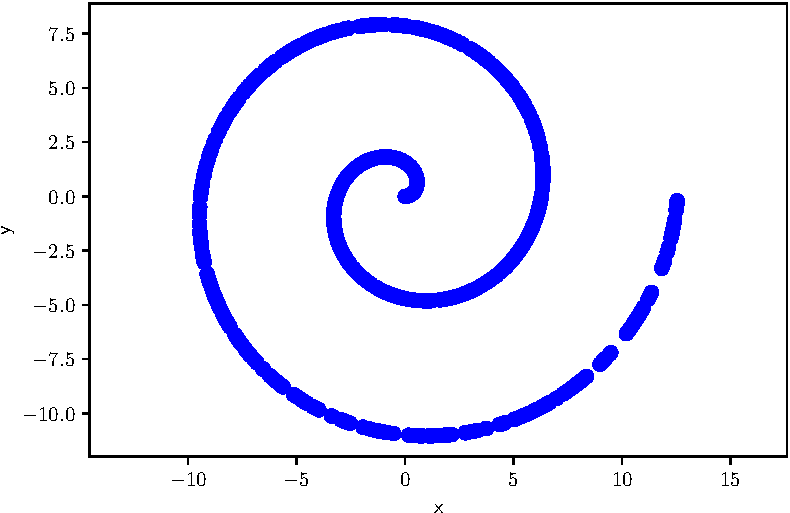
\includegraphics[width=0.6\columnwidth]{euc.pdf}
\end{center}
\caption{A spiral data set. The data is one-dimensional, if we know $x=r*cos(r)$, $y=r*sin(r)$.}
\vskip\baselineskip % Leave a vertical skip below the figure
\label{fig:spiral}
\end{figure}

Another important research direction in machine learning is \emph{unsupervised learning}. Here, we are not given a set of pre-defined targets. So we do not know the outcome of $\boldsymbol{y}$ that is dependent on the given input $\boldsymbol{x}$. We do not even know if there is any $\boldsymbol{y}$. The aim is to model the probability distribution of $\boldsymbol{x}$, to see what normally happens. Therefore the aim is to find statistical regularities within the $X$ space. However, without any supervision, it is not quite clear what is a statistical regularity. For example in Figure \ref{fig:spiral}, if we use Cartesian coordinates, we probably fail, or rather find poor estimates. If we know the transformation to polar coordinates, then we can model the distribution better by first transforming Cartesian coordinates to polar coordinates. Therefore, the transformation $\phi$ is the golden nugget.

The same argument is also true for supervised learning. However, we have the information that can direct us to find appropriate transformations: targets. Previously, people searched for better transformations to increase model performance. \emph{Deep learning} approach tries to solve the problem by also learning transformations. That is, we train a multi-layer perceptron (MLP), also called artificial neural network (ANN), to estimate $p(\boldsymbol{y}|\boldsymbol{x})$. The idea is to learn basic transformations at earlier layers and using them to construct higher level, more abstract transformations \cite{bengio2009}. When we learn abstract transformations from the data, we end up with models that have better \emph{generalization}, that is the performance on unseen data.

Supervised learning together with deep learning, achieved great success on real-world problems that requires generalization such as object recognition \cite{alexnet}, speech recognition \cite{acoustic} and statistical machine translation \cite{seq2seq}. Yet, the success of deep learning did not translate to unsupervised learning, until the proposal of \emph{generative adversarial networks} (GANs) \cite{gan}. While the label information may drive MLPs to learn abstract transformations, we do not have such information that directs us for unsupervised learning. The closest example is \emph{auto-encoders} (AEs).

% Deep neural networks (DNNs) have been shown to be very effective as discriminative models in real world tasks such as speech recognition \cite{acoustic}, object recognition \cite{alexnet} and machine translation \cite{seq2seq}. Generative adversarial networks (GAN) \cite{gan} and variational auto-encoders \cite{vae} (VAE) show that DNNs can also be used as generative models.

% There is also another approach called~\emph{unsupervised learning}. Here, we are not given a set of pre-defined targets. So we do not know the outcome of~$\boldsymbol{y}$~that is dependent on~$\boldsymbol{x}$. We do not even know what~$\boldsymbol{y}$~is. However, we assume that \emph{similar} outcomes of~$\boldsymbol{x}$~should yield similar outcomes of~$\boldsymbol{y}$. Therefore we focus on finding statistical regularities within~$X$. Once we know the structure of~$X$, it becomes considerably easy to find a mapping from~$X$~to~$Y$. Most important advantage of unsupervised learning algorithms is that they do not require labeled data. Therefore most of the time we can run our unsupervised algorithm with a vast amount of data and approximate the distribution of the population more accurately.



\chapter{GENERATIVE ADVERSARIAL NETWORKS}
\label{chapter:gan}

\section{Introduction}
\label{sec:gan:intro}

The generative adversarial network (GAN) \cite{gan}~has been proposed to learn a generative model to model a data distribution, $p(x)$. GAN is composed of two learners, a generative network $G$ and a discriminative network $D$. $G(z;\theta)$ learns to map $z$ sampled from an arbitrary distribution $p(z)$ to~the target distribution $p(x)$. It is a trained model, generally a deep neural network, parameterized by $\theta$. The discriminator $D(x;\phi)$, another neural network with weights $\phi$, is trained to assign low scores to ``fake'' samples generated $G(z;\theta)$ and high scores to samples from true $p(\boldsymbol{x})$ given in the training set.

GANs are used successfully especially in image generation. A well-trained GAN can generate images that are almost indistinguishable by humans \cite{stylegan}. Yet, there remain two main difficulties regarding the training: The first problem of mode collapse means that $G$ learns to generate some parts of $p(x)$ but not all; there are ways of being $x$ that cannot be generated for any $G(z)$. The second problem of vanishing gradients is because in practice both $D$ and $G$ are deep, and $G$ is doubly deep because its gradient needs to be back-propagated through $D$. Recent works mainly focus on these two problems. People proposed different GAN objectives, regularization methods, architectures and several other tricks \cite{ganreview}. The Wasserstein loss we use above is one example. 

The direction we pursue is to use multiple generators each one responsible from a local region of the $z$, and hence $x$ space. Different local generators will learn to cover different modes and this will help alleviate the mode collapse problem. We review three previously proposed approaches, namely multi-agent diverse GAN (MAD-GAN)\cite{madgan}, mixture GAN (MGAN)\cite{mgan}, and mixture of experts GAN (MEGAN)\cite{megan}. 

We propose the hierarchical mixture of generators, which learns a tree structure with internal decision nodes that divide up the input space and the leaves are local generators responsible from a local $z$ region generating a subset of $p(x)$. Since the splits are soft, given the tree structure, the parameters of the internal nodes as well as of the generators in the leaves can be updated using gradient-descent over Wasserstein loss. Note that it is only $G$ that is modeled this way, $D$ remains the usual deep neural network.

Generative adversarial network (GAN) is a neural network pair that tries to learn the data distribution $p(\boldsymbol{x})$ by playing a minimax game \cite{gan}. There are two networks, a generative network $G_{\theta}$ and a discriminative network $D_{\phi}$. We want $G_{\theta}$ to map an arbitrary distribution~$p(\boldsymbol{z})$~to~a target distribution~$p(\boldsymbol{x})$. Learning the set of parameters $\theta$ of $G_{\theta}$ is done by gradient descent. We provide the gradient information $\partial{G_{\theta}(\boldsymbol{z})} / \partial{\theta}$ by back-propagating the error from $D_{\phi}$. $D_{\phi}$ is trained to assign low probability to samples from $G_{\theta}(p(\boldsymbol{z}))$ and high probability to samples from $p(\boldsymbol{x})$. Here, $D_{\phi}$ can be thought as a teacher telling $G_{\theta}$ which way to go to get a better estimate. When $D_{\phi}$ becomes better, $G_{\theta}$ gets better instruction, therefore outputs better estimates. We can write the whole objective in a compact form as in \cite{gan}:

\begin{equation}
\label{eq:gan}
\mathbb{E}_{\boldsymbol{x} \sim p(\boldsymbol{x})} [ \log{D_{\phi}(\boldsymbol{x})} ] + 
\mathbb{E}_{\boldsymbol{z} \sim p(\boldsymbol{z})} [ \log{(1-D_{\phi}(G_{\theta}(\boldsymbol{x})))} ]
\end{equation} 

We try to minimize Equation \ref{eq:gan} for $G_{\theta}$ and maximize it for $D_{\phi}$.

The Wasserstein criterion \cite{wgan} is formulated as:
\begin{equation}
\mathbb{E}_{x\sim p(x} [D(x;\phi)] - 
    \mathbb{E}_{z\sim p(z)} [D(G(z;\theta);\phi)]
\label{eq:wgan}
\end{equation}

$D$ is trained to maximize this, i.e., it learns to maximize the difference between the expected score generated for the true samples in the training set and fake samples generated by $G$. At the same time, $G$ is trained to minimize this, i.e., it learns to generate fake samples that will be scored high by $D$. The parameters $\theta$ of $G$ and the parameters $\phi$ of $D$ are updated using gradient-descent/ascent. 

A well trained GAN can generate images that are almost indistinguishable by humans \cite{biggan,proggan,stylegan}. Yet, there remain difficulties regarding the training. Recently, Wassertein GAN \cite{wgan} proposed to minimize Earth-Mover distance (also known as Wasserstein-1 distance) instead of Jensen-Shannon divergence. They show both theoretically and experimentally that this loss has better convergence properties.

\section{Problems Related with GANs}
\label{sec:problems}

However, training of these architectures are notoriously hard. Two networks are trained simultaneously. Empirically, if $D_{\phi}$ is trained too much, then gradients that are propagated to $G_{\theta}$ become either too low or too high, depending on the use of original cost function or the non-saturating cost function \cite{principledmethods}. Another problem is when~$G_{\theta}$~quickly learns to generate a subset of~$p(\boldsymbol{x})$. Then again gradients that are propagated through~$D_{\phi}$~do not enforce~$G_{\theta}$~to generate diverse samples. This problem is called \emph{mode collapse}.

\section{Related Work}
\label{sec:related}

Recent works mainly focus on these two problems. To solve problems related to training people proposed different GAN objectives \cite{wgan,infogan,leastgan,lsgan}, regularization methods \cite{improved_wgan,sngan,dcgan}, architectures \cite{biggan,bigan,ali,proggan,stylegan,dcgan,sagan} and several other tricks mentioned in these papers. A good review of these works can be found in \cite{ganreview,ganreview2,ganreview3}.

The third main problem is the evaluation of models. Unlike Bayesian models where we can evaluate the quality of a model with marginal likelihood (or with evidence lower bounds), there is no proper way of evaluating GAN models.

For the evaluation of GAN methods, people seem to agree on Inception score (IS) \cite{improvedtechniques} and Fr\'echet Inception distance (FID) \cite{twotimes} since most of papers include these scores. Though it should be noted that these evaluation metrics are specifically for image domain. To the best of our knowledge, there is no work that generalizes these metrics to other domains. Other than these two methods, classifier two-sample test (C2ST) \cite{twosample} is a simple and effective way of evaluating GAN models. An extensive review of evaluation methods can be found in \cite{evalreview}.

Many unsupervised learning methods assume that $\boldsymbol{x}$~is determined by a set of factors $\boldsymbol{z}$ and an unpredictable noise factor $\epsilon$. So instead of finding $p(\boldsymbol{x})$, we try to find $p(\boldsymbol{z})$ and the mapping between $p(\boldsymbol{z})$ and $p(\boldsymbol{x})$. In the GAN framework, we generally fix $p(\boldsymbol{z})$ to be a spherical Gaussian distribution and let $G$~to find the relation between $p(\boldsymbol{z})$ and $p(\boldsymbol{x})$. Since DNNs are very powerful function approximators, we hope that $G$ can map $p(\boldsymbol{z})$ to $p(\boldsymbol{x})$ even if we fix $p(\boldsymbol{z})$. However, this mapping might be arbitrarily hard.

In this work, we use a soft decision tree (SDT) model \cite{sdt} in earlier layers of $G$, instead of a densely connected perceptron layer. Since an SDT is a continuous model, we can train the whole architecture with stochastic gradient descent (SGD). We experimentally show that our proposed architecture encapsulates the information in $p(\boldsymbol{z})$ in fewer dimensions with fewer trainable parameters. Furthermore, we can analyze the nodes of the tree after training to get an insight about $p(\boldsymbol{z})$.

Instead of trying to construct a different $p(\boldsymbol{z})$, one can learn different mappings for different regions of the input space. In multi-agent diverse GANs (MAD-GAN) \cite{madgan}, they propose to use multiple generators and force discriminator to also tell from which generator the data is generated.  MGAN \cite{mgan} is similar to MAD-GAN but they use a different classifier with parameters tied to discriminator network to classify generators. In mixture of experts GAN \cite{megan}, there are multiple generators but a gating function decides which generator to use based on features of generated data.

These works employ one shared generator with multiple generators at the end. This can be thought as transforming $p(\boldsymbol{z})$ to a representation that can be used by multiple models. We instead propose to transform $p(\boldsymbol{z})$ at the earlier layers then use a shared network to generate the data. By this way, generator can decide how to transform $p(\boldsymbol{z})$. Also, we can analyze the $p(\boldsymbol{z})$ after the training to see the relation between clusters in $p(\boldsymbol{z})$.

\chapter{MIXTURES OF GENERATORS}
\label{chapter:me}

\lipsum[5]

We use a widely adopted DCGAN \cite{dcgan} architecture for the generator. In DCGAN, we project the input noise vector $\boldsymbol{z}$ into a high dimensional vector and reshape it to apply transposed convolution operation. This projection is done with a fully-connected perceptron layer. Here, we remove this layer and add a SDT. Given an input vector $\boldsymbol{z}$, SDT softly decides which leaves (experts) to use. Leaves contain high-dimensional vectors (to be used for transposed convolution), that are also learned throughout the training. The model is visually summarized in Figure \ref{fig:tree}. Instead of a tree structure, a flat gating function can also be used as in \cite{me}.

Let $\boldsymbol{z} \in \mathbb{R}^{d}$. In the original DCGAN architecture, the data lies in $\mathbb{R}^{d}$ after the first transformation even though the resulting vector is high-dimensional. In our formulation, SDT can only output values in the \emph{convex hull} that is defined by its leaves since it takes a convex combination of its leaf values. Therefore, the data lies in $\mathbb{R}^m$ after the SDT transformation where $m$ is the number of leaves. As a result, we separate the relation between the dimensionality of the input vector and the latent distribution. For example, we can set the dimensionality of the noise vector as $2$ but have a $128$-dimensional latent distribution that is defined by the output of the SDT by using 128 leaves. The parameters of the gating functions and the leaves are learned throughout the training. The leaf values decide the vertices of the convex hull and the gating functions decide the distribution between the leaf values.

\section{Multi-Agent Diverse GAN}
\label{sec:madgan}

In MAD-GAN \cite{madgan} there are multiple generators and each generator labels the fake data with its index. The discriminator not only separates true examples from fakes, but also learns the index of the generator for a fake. This additional classification problem forces generators to be local.

\begin{figure}[htbp]
\begin{center}
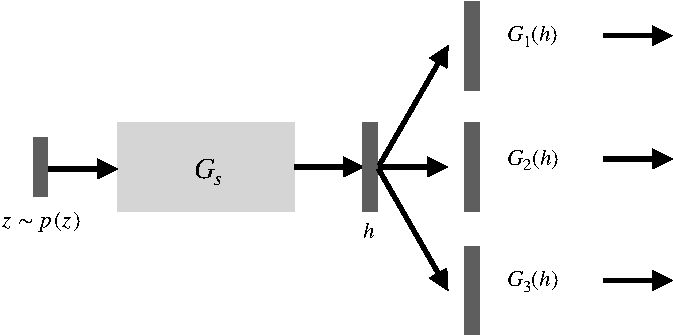
\includegraphics[width=0.75\columnwidth]{madgan.pdf}
\end{center}
\caption{Multi-agent diverse GAN}
\vskip\baselineskip % Leave a vertical skip below the figure
\label{fig:models:madgan}
\end{figure}

The model is shown in Figure \ref{fig:models:madgan}. Given $z$, a shared neural network block produces $z'$, an intermediate representation that is higher dimensional than $z$, which is used by a set of generators $\{G_i(z')\}_{i=1}^m$. The discriminator is a $m+1$-class classifier with 0 for true, and $1$ to $m$ for the fake instances. The discriminator should push the different generators to different modes to be able to solve the classification problem. 

%
%
\section{Mixture GAN}
\label{sec:mgan}

MGAN \cite{mgan} is similar to MAD-GAN except that the classifer and the discriminator are separate. The discriminator is two-class as usual discriminating between true and fake examples, and there is a separate $m$-class classifier only for the fake examples.

\begin{figure}[htbp]
\begin{center}
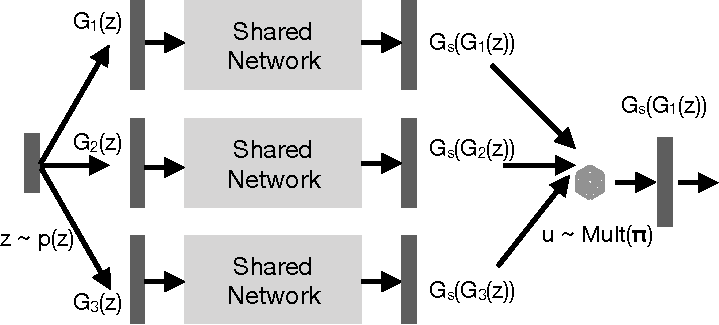
\includegraphics[width=0.75\columnwidth]{mgan.pdf}
\end{center}
\caption{Mixture GAN}
\vskip\baselineskip % Leave a vertical skip below the figure
\label{fig:models:mgan}
\end{figure}

The model is shown in Figure \ref{fig:models:mgan}. There is also the difference is that the split of the generators is earlier. A set of generators $\{G_i(z)\}_{i=1}^m$, transform $z$ and for all, the shared network produce $z'$. A multinomial distribution is sampled to randomly select one of the generators. While the discriminator tries to discriminate between fake and real data as usual, the classifier tries to predict the index of the generator that produced the fake sample. These two networks share parameters treating discriminator/classifier as a multi-task learning problem.

%
%
\section{Mixture of Experts GAN}
\label{sec:megan}

In the MEGAN \cite{megan}, inspired from the mixtures of experts \cite{me}, there is an additional gating model, which is also trained, that chooses among the different generators.

\begin{figure}[htbp]
\begin{center}
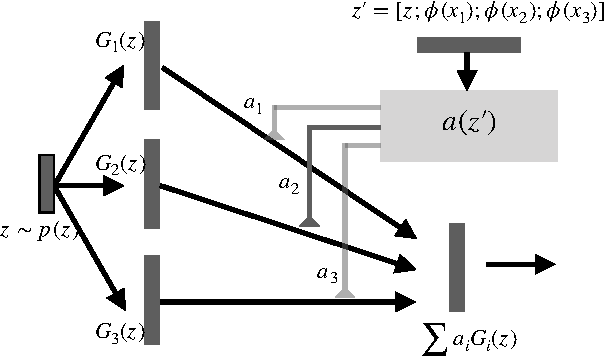
\includegraphics[width=0.75\columnwidth]{megan.pdf}
\end{center}
\caption{Mixture of experts GAN}
\vskip\baselineskip % Leave a vertical skip below the figure
\label{fig:models:megan}
\end{figure}

The model is shown in Figure \ref{fig:models:megan}. There is a set of generators $\{G_i(z)\}_{i=1}^{m}$ and an additional gating function, which takes as its input $z$ and some features from the generated $x$. Then Straight-Through Gumbel Softmax is applied which only selects one expert while allowing differentiability. The discriminator is still two-class. The gating model also has its parameters that are updated together with the generators. Although all generators generate an output, it is the gating model that decides which one is to be used. 

%
%
%
\chapter{HIERARCHICAL MIXTURE OF GENERATORS}
\label{chapter:hme}

A mixture of experts (ME) model consists of local experts $\{f_i(\boldsymbol{x})\}_{i=1}^{m}$, and a gating function $g(\boldsymbol{x})$ \cite{me}. Instead of learning a global function, we divide the input space into regions and learn a set of local functions. For a given input $\boldsymbol{x}$, the gating function outputs probabilities that decide which experts to use. Experts can be simple models since each expert needs to learn a local input-output mapping instead of a global one. The formal definition of the model is as follows:

\begin{eqnarray}
g(\boldsymbol{x}) = \text{softmax}(W_g \boldsymbol{x} + \boldsymbol{b}_g)\\
y = \sum_{i=1}^m g_i(\boldsymbol{x}) f_i(\boldsymbol{x})
\end{eqnarray}

where $y$ is the response of the model. Experts can be any differentiable function. It is recommended that we keep experts simple since we employ a multiple of them. For example, this can be a constant response, $f_i(\boldsymbol{x})=\boldsymbol{\rho}_i$, or a linear response, $f_i(\boldsymbol{x})=W_i \boldsymbol{x} + \boldsymbol{b}_i$.

In hierarchical mixtures of experts model (HME) \cite{hme}, we define a tree structure where internal nodes contain gating functions and leaves contain experts. The response of a binary tree node $m$ can be recursively defined as:

\begin{equation}
y_m(\boldsymbol{x})=
	\begin{cases}
		\hfil f_m(\boldsymbol{x}) &\text{if $m$ is a leaf} \\
		\hfil y_m^{L}(\boldsymbol{x})g_m(\boldsymbol{x}) + y_m^{R}(\boldsymbol{x})(1 - g_m(\boldsymbol{x})) &\text{otherwise}
	\end{cases}
\end{equation}

where $y_m^L$ and $y_m^R$ are the responses of the left and the right children of node $m$ respectively. This can be interpreted as a soft decision tree. In a hard decision tree, we either select the left child or the right child in a node whereas in a soft decision tree we take a convex combination of the child responses. One can fix the tree structure beforehand, or grow the tree adaptively based on the error \cite{sdt, budding}. Since the whole model is continuous, we can use gradient based optimization to learn the model parameters.

Just like the hierarchical mixture of experts \cite{hme} go from the flat organization of mixture of experts  \cite{me} to a tree, our proposed hierarchical mixture of generators go from a flat mixture of generators to a tree.

\begin{figure}[htbp]
\begin{center}
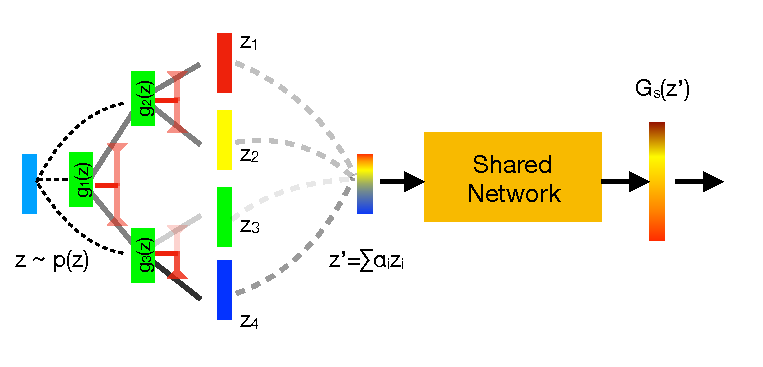
\includegraphics[width=0.75\columnwidth]{hmegan.pdf}
\end{center}
\caption{Hierarchical mixture of experts GAN}
\vskip\baselineskip % Leave a vertical skip below the figure
\label{fig:models:hmegan}
\end{figure}

As shown in Figure \ref{fig:models:hmegan}, we have a binary tree where each internal node has a gating model that chooses between the two children based on $z$. The leaves of the tree give the output $z'$. The final $z'$ is the weighted sum of all of the leaves weighted by the gating values on each path. A shared network then generates $x$ from this final $z'$. 

Since the whole model is continuous, one can use gradient based optimization to learn the parameters, which include all the gating parameters in all decision nodes in the tree as well as the $z'$ of all the leaves.

\chapter{EXPERIMENTS}
\label{chapter:exps}

\section{Data Sets}
\label{sec:datasets}

\section{Experimental Setup}
\label{sec:setup}

\section{Hierarchical Structure vs. Flat Structure}
\label{sec:hme-vs-me}

\section{Fully-connected vs. HME}
\label{sec:fc-vs-hme}

\section{Linear Experts}
\label{sec:hme-linear}

\section{Interpretation of the Learned Model}
\label{sec:interpret}

We test our proposed mixture model on four image data sets that are widely used in GAN literature, namely, MNIST \cite{mnist}, FashionMNIST \cite{fashion}, UTZap50K \cite{utzap50k} and CelebA \cite{celeba}. 

We use trees of different depths, and we also test a flat mixture of generators of equal number of leaves. For example, we have a tree of depth five with 32 leaves and a flat mixture of 32 leaves. In the former case, for each leaf, we have five binary gatings; in the latter case, there is one gating that chooses one of 32. 

We test these against a fully connected (FC) layer. In Figure \ref{fig:models:hmegan}, this corresponds to having one fully connected layer between $z$ and $z'$. One advantage of the gating lies in complexity. Let us say $z$ is 100 dimensional and $z'$ is 1000 dimensional; a fully connected layer has 100 000 weights, but a tree uses gating nodes all of which are 100 dimensional, so unless the tree has more than 100 leaves, the tree is much simpler in terms of memory and computation.

\begin{table}[thbp]
\vskip\baselineskip
\caption{Deconvolution network architectures that are used. The small network is used on MNIST and FashionMNIST which are $32\times 32$ and the large is used on UTZap50K and CelebA which are $64\times 64$.}
\begin{center}
\begin{tabular}{|l|c|c|}
\hline
\textbf{Layer} & \textbf{Small Network} & \textbf{Large Network}\\
 \hline
1 & 100                    & 100 \\
 \hline
2 &  $256 \times 4 \times 4$ & $512 \times 4 \times 4$\\
\hline
3 & $128 \times 8 \times 8$ & $256 \times 8 \times 8$\\
\hline
4 & $64 \times 16 \times 16$& $128 \times 16 \times 16$\\
 \hline
5 & $ 1 \times 32 \times 32$& $64 \times 32 \times 32$\\
 \hline
6 & - & $3 \times 64 \times 64$\\
 \hline
\end{tabular}
\label{tab:models}
\end{center}
\end{table}

The convolutional architecture that we use is the DCGAN \cite{dcgan}. We resized MNIST and FashionMNIST to $32\times 32$ pixels and other data sets to $64\times 64$ pixels. The network architectures used for the former and latter data sets are given in Table \ref{tab:models} that shows the number of units in each layer and the convolutional structure. Layers 2 to 5 are transposed convolutional layers and layer 1 is fully connected for FC, or is where we have the HME or ME structure embedded. 

Wasserstein loss \cite{wgan} with gradient penalty \cite{improved_wgan} is used throughout all experiments, and we adopted the suggested hyperparameter setting of Wasserstein loss recommended in \cite{improved_wgan}. The dimensionality of the input $z$ is set to 100. For the hierarchical model, we tested trees with depth 5, 6 and 7. To get the same number of leaves, we used 32, 64, and 128 generator experts in the flat mixture. 

For the evaluation of GAN methods, we used the most popular evaluation criteria that are the Fr\'echet Inception distance (FID) \cite{twotimes} and the two-sample test (C2ST) \cite{twosample}, here, 5-nearest neighbor (5-NN) leave-one-out accuracy. Both FID and 5-NN accuracy are calculated with the activations before the softmax layer (2048-dim) of InceptionV3 \cite{inceptionv3}. All models are run five times with different random seeds, and we report the average and standard deviations. Lower FID scores are better and 5-NN accuracies that are close to 50\% are better. 

\begin{figure}[htbp]
\begin{center}
\subfloat[MNIST]{
	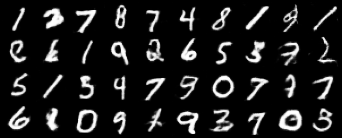
\includegraphics[width=0.6\linewidth]{mnist_samples.png}
	\label{fig:samples:mnist}
}

\subfloat[FashionMNIST]{
	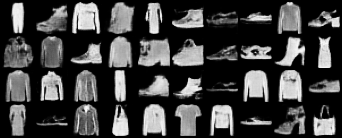
\includegraphics[width=0.6\linewidth]{fashion_samples.png}
	\label{fig:samples:fashion}
}

\subfloat[UTZap50K]{
	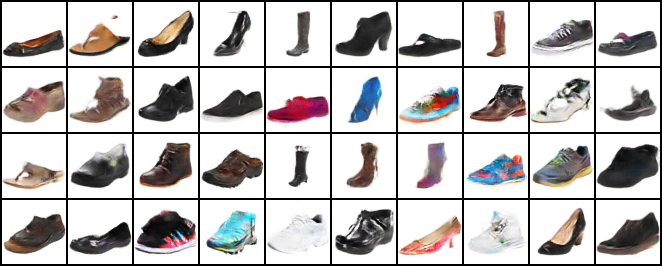
\includegraphics[width=0.6\linewidth]{shoes_samples.png}
	\label{fig:samples:shoes}
}

\subfloat[CelebA]{
	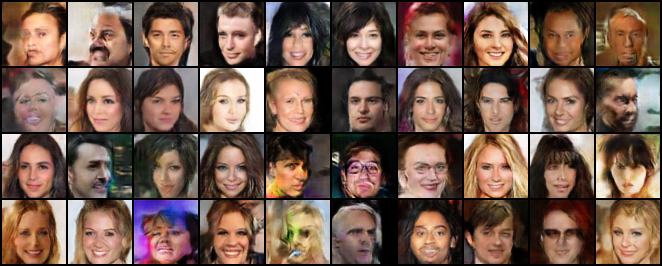
\includegraphics[width=0.6\linewidth]{celeba_samples.png}
	\label{fig:samples:celeba}
}
\end{center}
\caption{Samples generated using our proposed hierarchical mixture of generators.}
\vskip\baselineskip
\label{fig:samples}
\end{figure}

Some generated examples for different data sets using the hierarchical mixture model are shown in Figure \ref{fig:samples}. It can be seen that these are quite realistic and contain diversity. Here, we use a tree with depth 5 for all data sets, except FashionMNIST where we use a tree with depth 7.

\begin{table}[thbp]
\vskip\baselineskip
\caption[Results of FC and HME models]{Results of FC and HME models. $dim(\boldsymbol{z})$ is fixed to 100.}
\begin{center}
\begin{tabular}{|p{0.2cm}|p{0.2cm}|c|c|c|c|c|}
\cline{3-7}
\multicolumn{2}{c|}{} & FC		& HME-5		& HME-6		& HME-7		& HME-8		\\
\hline
\multirow{3}{*}{\rotatebox{90}{MNIST}}
& \rotatebox{90}{Real} & $74.90 \pm 0.59$ & $73.62 \pm 0.91^-$ & $73.70 \pm 0.54^-$ &  {$73.27 \pm 0.48^-$} &  {$73.39 \pm 0.47^-$} \\
\cline{2-7}
& \rotatebox{90}{Fake} & $67.89 \pm 0.30$ & $73.24 \pm 1.03^+$ & $72.00 \pm 1.10^+$ &  {$70.97 \pm 0.35^+$} &  {$71.20 \pm 0.48^+$} \\
\cline{2-7}
& \rotatebox{90}{FID} & $11.13 \pm 0.44$ & $13.57 \pm 0.31^+$ & $12.61 \pm 0.84^+$ & $11.93 \pm 0.44^+$ & {$11.84 \pm 0.48^+$} \\
\hline
\multicolumn{2}{|c|}{\#} & 413K & 134K & 268K & 537K & 1.07M \\
\hline
\multirow{3}{*}{\rotatebox{90}{Fashion}}
& \rotatebox{90}{Real} & $75.01 \pm 0.20$ & $73.46 \pm 0.68^-$ & $73.22 \pm 0.86^-$ & $73.14 \pm 1.47^-$ & $72.45 \pm 2.08$ \\
\cline{2-7}
& \rotatebox{90}{Fake} & $84.89 \pm 0.39$ & $89.32 \pm 0.72^+$ & {$88.36 \pm 0.95^+$} & {$87.47 \pm 1.14^+$} & {$86.95 \pm 1.27^+$} \\
\cline{2-7}
& \rotatebox{90}{FID} & $26.50 \pm 0.63$ & $27.92 \pm 0.91^+$ & $26.85 \pm 1.35$ & $25.93 \pm 1.48$ & {$25.51 \pm 2.41$} \\
\hline
\multicolumn{2}{|c|}{\#} & 413K & 134K & 268K & 537K & 1.07M \\
\hline
\multirow{3}{*}{\rotatebox{90}{CelebA}}
& \rotatebox{90}{Real} & $66.14 \pm 1.17$ & $72.16 \pm 0.51^+$ & $70.35 \pm 0.63^+$ & $68.61 \pm 0.81^+$ & $68.96 \pm 1.39^+$ \\
\cline{2-7}
& \rotatebox{90}{Fake} & $80.96 \pm 1.56$ & $91.14 \pm 0.40^+$ & $89.93 \pm 0.15^+$ & $87.71 \pm 0.95^+$ & $88.12 \pm 0.62^+$ \\
\cline{2-7}
& \rotatebox{90}{FID} & $14.93 \pm 0.48$ & $21.40 \pm 0.61^+$ & $19.97 \pm 0.27^+$ & $18.21 \pm 0.52^+$ & $18.20 \pm 0.47^+$ \\
\hline
\multicolumn{2}{|c|}{\#} & 827K & 265K & 530K & 1.06M & 2.12M \\
\hline
\multirow{3}{*}{\rotatebox{90}{UTZap50K}}
& \rotatebox{90}{Real} & $89.59 \pm 1.40$ & $91.64 \pm 0.83^+$ & $90.62 \pm 0.59$ & $90.47 \pm 0.70$ & $90.30 \pm 0.73$ \\
\cline{2-7}
& \rotatebox{90}{Fake} & $81.51 \pm 1.16$ & $86.02 \pm 0.67^+$ & $85.13 \pm 0.46^+$ & {$84.02 \pm 0.43^+$} & {$83.71 \pm 0.61^+$} \\
\cline{2-7}
& \rotatebox{90}{FID} & $54.48 \pm 5.36$ & $63.67 \pm 3.40^+$ & $58.96 \pm 1.28$ & $57.43 \pm 3.06$ & {$56.48 \pm 2.39$} \\
\hline
\multicolumn{2}{|c|}{\#} & 827K & 265K & 530K & 1.06M & 2.12M \\
\hline
\multirow{3}{*}{\rotatebox{90}{Flowers}}
& \rotatebox{90}{Real} & $93.80 \pm 1.02$ & $93.83 \pm 0.95$ & $93.41 \pm 0.96$ & $93.14 \pm 0.83$ & $93.38 \pm 0.96$ \\
\cline{2-7}
& \rotatebox{90}{Fake} & $97.60 \pm 0.71$ & $97.48 \pm 0.48$ & {$97.42 \pm 0.35$} & $97.46 \pm 0.58$ & $97.24 \pm 0.74$ \\
\cline{2-7}
& \rotatebox{90}{FID} & $135.28 \pm 7.28$ & $133.47 \pm 6.22$ & $131.05 \pm 4.61$ & $128.95 \pm 3.49$ & $128.62 \pm 5.94$ \\
\hline
\multicolumn{2}{|c|}{\#} & 827K & 265K & 530K & 1.06M & 2.12M \\
\hline
\end{tabular}
\label{tab:fc-hme}
\end{center}
\end{table}

\begin{table}[thbp]
\vskip\baselineskip
\caption[Results for ME models]{Results for ME models. $dim(\boldsymbol{z})$ is fixed to 100.}
\begin{center}
\begin{tabular}{|c|c|c|c|c|c|}
\cline{3-6}
\multicolumn{2}{c|}{} & ME-32		& ME-64		& ME-128		& ME-256 \\
\hline
\multirow{3}{*}{\rotatebox{90}{MNIST}}
& \rotatebox{90}{Real} & $74.23 \pm 0.58$ & $74.00 \pm 0.31^-$ & $74.57 \pm 0.86$ & $76.31 \pm 0.79^+$ \\
\cline{2-6}
& \rotatebox{90}{Fake} & $74.11 \pm 0.77^+$ & $72.12 \pm 0.74^+$ & $72.65 \pm 1.30^+$ & $72.97 \pm 0.52^+$ \\
\cline{2-6}
& \rotatebox{90}{FID} & $13.71 \pm 1.19^+$ & $12.08 \pm 0.23^+$ & $12.75 \pm 0.77^+$ & $14.58 \pm 1.10^+$ \\
\hline
\multicolumn{2}{|c|}{params.} & 134K & 268K & 537K & 1.07M \\
\hline
\multirow{3}{*}{\rotatebox{90}{Fashion}}
& \rotatebox{90}{Real} & $74.05 \pm 0.81$ & $73.54 \pm 1.10^-$ & $75.84 \pm 2.43$ & $75.63 \pm 2.48$ \\
\cline{2-6}
& \rotatebox{90}{Fake} & $90.23 \pm 0.47^+$ & $90.31 \pm 0.59^+$ & $90.50 \pm 1.47^+$ & $90.46 \pm 1.65^+$ \\
\cline{2-6}
& \rotatebox{90}{FID} & $27.68 \pm 0.83^+$ & $27.86 \pm 1.34$ & $28.47 \pm 2.90$ & $29.49 \pm 2.86$ \\
\hline
\multicolumn{2}{|c|}{params.} & 134K & 268K & 537K & 1.07M \\
\hline
\multirow{3}{*}{\rotatebox{90}{CelebA}}
& \rotatebox{90}{Real} & $72.22 \pm 1.60^+$ & $71.23 \pm 1.07^+$ & $69.66 \pm 0.84^+$ & $69.23 \pm 1.29^+$ \\
\cline{2-6}
& \rotatebox{90}{Fake} & $91.04 \pm 1.86^+$ & $90.56 \pm 1.87^+$ & $87.92 \pm 0.48^+$ & $87.83 \pm 0.66^+$ \\
\cline{2-6}
& \rotatebox{90}{FID} & $20.96 \pm 0.78^+$ & $20.27 \pm 0.70^+$ & $18.78 \pm 0.35^+$ & $18.39 \pm 0.76^+$ \\
\hline
\multicolumn{2}{|c|}{params.} & 265K & 530K & 1.06M & 2.12M \\
\hline
\multirow{3}{*}{\rotatebox{90}{UTZap50K}}
& \rotatebox{90}{Real} & $91.07 \pm 0.62$ & $91.18 \pm 0.34$ & $90.95 \pm 0.82$ & $91.31 \pm 1.18$ \\
\cline{2-6}
& \rotatebox{90}{Fake} & $86.69 \pm 1.18^+$ & $85.67 \pm 0.99^+$ & $85.38 \pm 0.42^+$ & $86.06 \pm 1.04^+$ \\
\cline{2-6}
& \rotatebox{90}{FID} & $63.72 \pm 4.35^+$ & $61.19 \pm 2.02^+$ & $61.51 \pm 2.52^+$ & $65.19 \pm 3.85^+$ \\
\hline
\multicolumn{2}{|c|}{params.} & 265K & 530K & 1.06M & 2.12M \\
\hline
\multirow{3}{*}{\rotatebox{90}{Flowers}}
& \rotatebox{90}{Real} & $93.58 \pm 1.26$ & $93.69 \pm 0.50$ & $93.57 \pm 1.41$ & $94.40 \pm 1.19$ \\
\cline{2-6}
& \rotatebox{90}{Fake} & $97.88 \pm 0.58$ & $97.96 \pm 0.30$ & $97.76 \pm 0.41$ & $97.89 \pm 0.48$ \\
\cline{2-6}
& \rotatebox{90}{FID} & $133.13 \pm 4.31$ & $131.83 \pm 2.45$ & $132.07 \pm 7.28$ & $137.08 \pm 6.46$ \\
\hline
\multicolumn{2}{|c|}{params.} & 265K & 530K & 1.06M & 2.12M \\
\hline
\end{tabular}
\label{tab:me}
\end{center}
\end{table}


\begin{table}[thbp]
\vskip\baselineskip
\caption[HME with linear experts for different tree depths]{HME with linear experts for different tree depths. $dim(\boldsymbol{z})$ is fixed to 32.}
\begin{center}
\begin{tabular}{|c|c|c|c|c|c|}
\hline
\multicolumn{2}{|c|}{Depth} & 2 & 3 & 4 & 5 \\
\hline
\multirow{3}{*}{\rotatebox{90}{MNIST}}
& \rotatebox{90}{Real} & $73.75 \pm 0.61$ & $71.83 \pm 0.77$ & $71.43 \pm 0.32$ & $70.81 \pm 0.39$ \\
\cline{2-6}
& \rotatebox{90}{Fake} & $66.07 \pm 0.89$ & $65.30 \pm 0.89$ & $65.30 \pm 0.59$ & $65.05 \pm 0.65$ \\
\cline{2-6}
& \rotatebox{90}{FID} & $9.98 \pm 0.60$ & $8.91 \pm 0.47$ & $8.71 \pm 0.32$ & $8.46 \pm 0.28$ \\
\hline
\multicolumn{2}{|c|}{params.} & 540K & 1.08M & 2.16M & 4.32M \\
\hline
\multirow{3}{*}{\rotatebox{90}{Fashion}}
& \rotatebox{90}{Real} & $70.85 \pm 0.67$ & $69.52 \pm 0.46$ & $68.55 \pm 0.61$ & $69.08 \pm 0.64$ \\
\cline{2-6}
& \rotatebox{90}{Fake} & $78.53 \pm 0.38$ & $78.46 \pm 0.21$ & $77.64 \pm 0.90$ & $78.27 \pm 1.29$ \\
\cline{2-6}
& \rotatebox{90}{FID} & $19.40 \pm 0.79$ & $18.57 \pm 0.52$ & $17.75 \pm 0.58$ & $18.01 \pm 0.73$ \\
\hline
\multicolumn{2}{|c|}{params.} & 540K & 1.08M & 2.16M & 4.32M \\
\hline
\multirow{3}{*}{\rotatebox{90}{CelebA}}
& \rotatebox{90}{Real} & $62.48 \pm 1.27$ & $78.26 \pm 1.08$ & $62.60 \pm 1.20$ & $61.73 \pm 0.94$ \\
\cline{2-6}
& \rotatebox{90}{Fake} & $78.64 \pm 1.09$ & $62.20 \pm 1.28$ & $78.84 \pm 0.69$ & $77.72 \pm 0.46$ \\
\cline{2-6}
& \rotatebox{90}{FID} & $12.58 \pm 0.41$ & $12.46 \pm 0.69$ & $12.79 \pm 	0.43$ & $12.03 \pm 0.25$ \\
\hline
\multicolumn{2}{|c|}{params.} & 1.08M & 2.16M & 4.32M & 8.65M \\
\hline
\multirow{3}{*}{\rotatebox{90}{UTZap50K}}
& \rotatebox{90}{Real} & $86.27 \pm 1.08$ & $86.18 \pm 0.99$ & $86.04 \pm 0.75$ & $86.49 \pm 0.71$ \\
\cline{2-6}
& \rotatebox{90}{Fake} & $77.10 \pm 0.88$ & $78.86 \pm 0.69$ & $76.62 \pm 0.78$ & $77.25 \pm 0.92$ \\
\cline{2-6}
& \rotatebox{90}{FID} & $40.19 \pm 2.79$ & $40.04 \pm 2.30$ & $38.83 \pm 0.80$ & $40.88 \pm 2.13$ \\
\hline
\multicolumn{2}{|c|}{params.} & 1.08M & 2.16M & 4.32M & 8.65M \\
\hline
\multirow{3}{*}{\rotatebox{90}{Flowers}}
& \rotatebox{90}{Real} & $89.50 \pm 2.25$ & $88.24 \pm 0.84$ & $89.39 \pm 1.02$ & $89.08 \pm 1.71$ \\
\cline{2-6}
& \rotatebox{90}{Fake} & $95.62 \pm 0.90$ & $95.94 \pm 0.90$ & $96.24 \pm 0.28$ & $96.28 \pm 0.67$ \\
\cline{2-6}
& \rotatebox{90}{FID} & $109.97 \pm 7.29$ & $107.81 \pm 4.21$ & $112.73 \pm 4.55$ & $109.88 \pm 4.28$ \\
\hline
\multicolumn{2}{|c|}{params.} & 1.08M & 2.16M & 4.32M & 8.65M \\
\hline
\end{tabular}
\label{tab:hme-depth}
\end{center}
\end{table}

\begin{table}[thbp]
\vskip\baselineskip
\caption[HME with linear experts for embedding spaces with different dimensionalities]{HME with linear experts for embedding spaces with different dimensionalities. Depth is fixed to 5.}
\begin{center}
\begin{tabular}{|c|c|c|c|c|c|}
\hline
\multicolumn{2}{|c|}{$dim(\boldsymbol{z})$} & 4 & 32 & 64 & 100 \\
\hline
\multirow{3}{*}{\rotatebox{90}{MNIST}}
& \rotatebox{90}{Real} & $74.94 \pm 0.67$ & $70.81 \pm 0.39^-$ & $71.27 \pm 0.46^-$ & $72.14 \pm 0.54^-$ \\
\cline{2-6}
& \rotatebox{90}{Fake} & $86.88 \pm 0.65^+$ & $65.05 \pm 0.65^-$ & $65.33 \pm 0.60^-$ & $65.63 \pm 0.25^-$ \\
\cline{2-6}
& \rotatebox{90}{FID} & $17.42 \pm 0.88^+$ & $8.46 \pm 0.28^-$ & $8.55 \pm 0.25^-$ & $9.07 \pm 0.44^-$ \\
\hline
\multicolumn{2}{|c|}{params.} & 655K & 4.32M & 8.52M & 13.24M \\
\hline
\multirow{3}{*}{\rotatebox{90}{Fashion}}
& \rotatebox{90}{Real} & $73.33 \pm 0.87^-$ & $69.08 \pm 0.64^-$ & $69.62 \pm 0.87^-$ & $69.99 \pm 0.70^-$ \\
\cline{2-6}
& \rotatebox{90}{Fake} & $96.62 \pm 0.44^+$ & $78.27 \pm 1.29^-$ & $77.99 \pm 0.70^-$ & $78.10 \pm 0.60^-$ \\
\cline{2-6}
& \rotatebox{90}{FID} & $28.37 \pm 1.40^+$ & $18.01 \pm 0.73^-$ & $18.32 \pm 0.67^-$ & $18.24 \pm 0.91^-$ \\
\hline
\multicolumn{2}{|c|}{params.} & 655K & 4.32M & 8.52M & 13.24M \\
\hline
\multirow{3}{*}{\rotatebox{90}{CelebA}}
& \rotatebox{90}{Real} & $75.88 \pm 0.83^+$ & $61.73 \pm 0.94^-$ & $61.91 \pm 0.72^-$ & $62.02 \pm 1.02^-$ \\
\cline{2-6}
& \rotatebox{90}{Fake} & $98.10 \pm 0.26^+$ & $77.72 \pm 0.46^-$ & $77.14 \pm 0.83^-$ & $77.02 \pm 0.98^-$ \\
\cline{2-6}
& \rotatebox{90}{FID} & $26.21 \pm 0.38^+$ & $12.03 \pm 0.25^-$ & $11.99 \pm 0.40^-$ & $12.09 \pm 0.56^-$ \\
\hline
\multicolumn{2}{|c|}{params.} & 1.31M & 8.65M & 17.04M & 26.47M \\
\hline
\multirow{3}{*}{\rotatebox{90}{UTZap50K}}
& \rotatebox{90}{Real} & $92.45 \pm 0.47^+$ & $86.49 \pm 0.71^-$ & $85.98 \pm 0.87^-$ & $87.77 \pm 1.17$ \\
\cline{2-6}
& \rotatebox{90}{Fake} & $91.39 \pm 0.66^+$ & $77.25 \pm 0.92^-$ & $76.40 \pm 1.08^-$ & $78.42 \pm 1.36^-$ \\
\cline{2-6}
& \rotatebox{90}{FID} & $70.91 \pm 4.65^+$ & $40.88 \pm 2.13^-$ & $38.79 \pm 2.26^-$ & $45.54 \pm 3.46^-$ \\
\hline
\multicolumn{2}{|c|}{params.} & 1.31M & 8.65M & 17.04M & 26.47M \\
\hline
\multirow{3}{*}{\rotatebox{90}{Flowers}}
& \rotatebox{90}{Real} & $94.13 \pm 1.08$ & $89.08 \pm 1.71^-$ & $88.30 \pm 1.21^-$ & $90.15 \pm 1.60^-$ \\
\cline{2-6}
& \rotatebox{90}{Fake} & $98.16 \pm 0.29$ & $96.28 \pm 0.67^-$ & $96.77 \pm 0.65$ & $96.55 \pm 0.76$ \\
\cline{2-6}
& \rotatebox{90}{FID} & $133.34 \pm 1.24$ & $109.88 \pm 4.28^-$ & $110.93 \pm 4.54^-$ & $114.79 \pm 4.20^-$ \\
\hline
\multicolumn{2}{|c|}{params.} & 1.31M & 8.65M & 17.04M & 26.47M \\
\hline
\end{tabular}
\label{tab:hme-zdim}
\end{center}
\end{table}

Experiment results are reported in Table \ref{tab:fc-hme}. HME-$k$ refers to a tree with depth $k$ and ME-$k$ refers to $k$ experts. We report the parameter count of FC, HME and ME; these do not include the convolution parameters shared across all models. These results show that HME and ME, though are good, are not as good as FC in terms of Frechet score or 5-NN accuracy. Their performance improves as the structure gets larger; note that trees with depth 5 and 6 are smaller than FC.

\begin{figure}[htbp]
\begin{center}
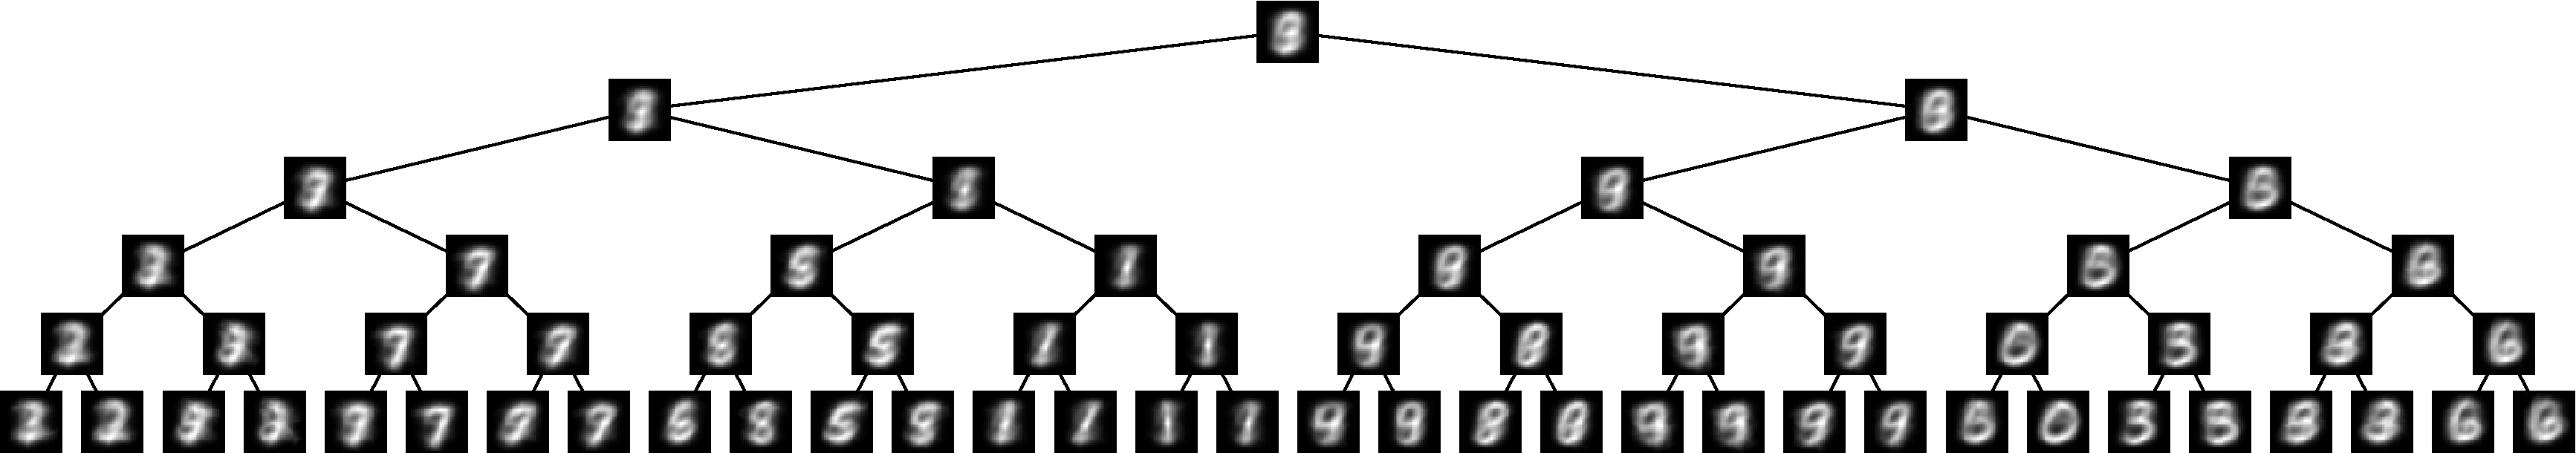
\includegraphics[width=\columnwidth]{tree_mnist.pdf}
\end{center}
\caption{Mean responses of each node. As we go down in the tree, granularity level increases.}
\vskip\baselineskip % Leave a vertical skip below the figure
\label{fig:tree}
\end{figure}

Though our proposed model is not as good as the FC in terms of FID or 5-NN scores, its main advantage is interpretability. To investigate the learned representation, we generate $100$ samples from the generated model and for each node $m$, we take a weighted average of the generated samples. In a hard decision tree where we choose left or right, a hard count corresponds to the path from root to prediction leaf. Here, we instead find the soft count of a node by multiplying the gating values up to that node. The result is visualized in Figure \ref{fig:tree}. We see that earlier levels of the tree correspond to the means of larger samples and as we go down to the leaves, there is specialization, an indication that the tree structure divides the input space into regions. We can think of the structure implementing a soft hierarchical clustering. 

\chapter{CONCLUSION}
\label{chapter:conc}
We propose a hierarchical mixture of generators model for GAN. We show that the parameters can be trained using the gradient information. Our experimental results show that the model can generate samples that are realistic and diverse. Though results are not as good as the the fully connected vanilla model, they are promising.

The greatest advantage of the proposed model is interpretability. Since this is a tree architecture, we can make post-hoc analysis to the learned tree to gain insight about the data. The tree structure indicates granularity at different levels and leaves correspond to modes of the distribıtion.

One future direction is to increase complexity at the leaf level; instead of constant leaves as we have now, we can have linear leaves. Another direction is to adapt the tree structure, that is model complexity, as well as parameters, during learning.

\bibliographystyle{styles/fbe_tez_v11}
\bibliography{references}

\end{document}